\section{Multistrand Common-Terminal Circuits and Sharing Criterion}
\label{chapter:04}

% block-id: 04.common.heading
\hypertarget{04.common.heading}{}
\subsection{Common-terminal coupling and uniform complex currents}

% block-id: 04.common.p1
\hypertarget{04.common.p1}{}
The common endpoints, strand branches, and return are related in Fig.~\ref{fig:common_terminal}. Let Z be the coupled impedance matrix of a specified linear model, e the independently induced voltage, i the complex strand currents, and V the common terminal voltage. The port equation Zi+e=V1 and total-current constraint 1\(^{\mathrm T}\)i=It form \eqref{eq:E04}. Solving the augmented system yields both magnitude and phase; It/N serves as a reference for the resulting current distribution.

% block-id: 04.common.p2
\hypertarget{04.common.p2}{}
When the augmented system has a unique solution, substitution of i=(It/N)1 shows that uniform currents exist if and only if every component of (It/N)Z1+e is equal. Projecting this vector onto the subspace orthogonal to 1 gives \eqref{eq:E05}. Without an independent imposed field, the condition reduces to equal row sums of Z; with an imposed field, the induced term also determines current sharing. This necessary and sufficient condition applies to the selected impedance model and terminal conditions, expressing the effect of transposition through changes in coupling and induced voltages.

% block-id: 04.common.p3
\hypertarget{04.common.p3}{}
The two-dimensional common-terminal FEM solves the shared axial terminal field jointly with Az degrees of freedom. In conductors, Jz=σ(v−u), where both v and the saved variable u are expressed in V/m; the return conductor uses its corresponding terminal field. Current and loss are integrated on material-tagged linear triangles after coordinates are converted from mm to m. Strand currents, bundle loss, return loss, and copper area are independently compared with the original field–circuit results, treating air and conductor regions separately.

% block-id: 04.sharing_derivation.heading
\hypertarget{04.sharing_derivation.heading}{}
\subsection{Derivation of the uniform complex-current condition}

% block-id: 04.sharing_derivation.p1
\hypertarget{04.sharing_derivation.p1}{}
If a uniform-current solution exists, substituting i=(It/N)1 into the port equation makes all components of (It/N)Z1+e equal, establishing necessity of the projection condition. Conversely, when the projection condition holds, this vector equals a scalar V times 1. The uniform-current vector then satisfies both the port equation and the total-current constraint; uniqueness of the augmented solution makes it the actual solution, establishing sufficiency. Numerical results use sqrt(mean(|ik−It/N|²))/|It/N| for normalized RMS complex-current deviation and show individual magnitudes and phases.

% block-id: 04.coax_results.heading
\hypertarget{04.coax_results.heading}{}
\subsection{Common-terminal currents and loss in a 640-strand straight bundle}

% block-id: 04.coax_results.p1
\hypertarget{04.coax_results.p1}{}
Three meshes and variations of return distance and exterior domain complete 23 checks. The final mesh refinement changes Rac by 0.011902\%; return-distance and exterior-domain changes are 0.000495\% and 0.000270\%, respectively, as shown in Fig.~\ref{fig:coax640_mesh}. These changes remain below the 1\% comparison target over the tested perturbations, supporting numerical stability of the specified two-dimensional common-terminal result. Its applicability is a straight two-dimensional bundle with a controlled return; finite end regions and longitudinal coupling in actual wound structures require further verification.

% block-id: 04.coax_results.p2
\hypertarget{04.coax_results.p2}{}
Fig.~\ref{fig:coax640_currents} shows current magnitude and phase by physical strand identity, with It/N as the equal-current reference. Magnitude and phase jointly determine each strand's contribution to total transport current, so current sharing is evaluated using complex currents. Fig.~\ref{fig:coax640_fields} gives the corresponding cross-sectional fields, connecting strand statistics with spatial position. In this axially invariant straight bundle, the skin-effect scale within each fine strand coexists with collective current redistribution caused by magnetic coupling across the bundle. Longitudinal transposition requires a separate representation of position changes.

% block-id: 04.interpretation.heading
\hypertarget{04.interpretation.heading}{}
\subsection{Interpretation}

% block-id: 04.interpretation.p1
\hypertarget{04.interpretation.p1}{}
The 640-strand section distinguishes the skin-effect scale of an individual fine strand from collective current redistribution in the bundle. Inner and outer strands experience different magnetic coupling; under a common terminal field, this difference appears in current magnitude and phase. DC area supplies a reference for copper utilization, the bundle Joule integral gives transport loss, and the separate return integral describes energy allocation across the complete field–circuit system.

% block-id: 04.quantitative.p1
\hypertarget{04.quantitative.p1}{}
The actual copper cross-section of the two-dimensional 640-strand model is \metric{coax_area} mm². Bundle AC resistance is \metric{coax_rac} mΩ per axial metre, bundle loss is \metric{coax_bundle_loss} W per axial metre, and return loss is \metric{coax_return_loss} W per axial metre. Separate integration identifies dissipation in the bundle and return. The common axial terminal field is \metric{coax_voltage_re}+j(\metric{coax_voltage_im}) V/m. Complex strand currents sum to 20 A RMS, while their normalized RMS complex-current deviation is \metric{coax_spread}, demonstrating substantial interstrand differences in this common-terminal straight bundle.

% block-id: 04.equation.E04
\hypertarget{04.equation.E04}{}
\hypertarget{E04}{}\begin{equation}\begin{bmatrix} Z&-\mathbf1\\ \mathbf1^T&0\end{bmatrix}\begin{bmatrix}\mathbf i\\V\end{bmatrix}=\begin{bmatrix}-\mathbf e\\I_t\end{bmatrix}\tag{4}\label{eq:E04}\end{equation}

% block-id: 04.equation.E05
\hypertarget{04.equation.E05}{}
\hypertarget{E05}{}
\begin{equation}
\begin{gathered}
Q=I_N-\mathbf1\mathbf1^T/N \\
Q\left[(I_t/N)Z\mathbf1+\mathbf e\right]=\mathbf0
\end{gathered}
\tag{5}\label{eq:E05}
\end{equation}

% block-id: 04.figure.common_terminal
\hypertarget{04.figure.common_terminal}{}
\begin{figure}[!htbp]
\centering
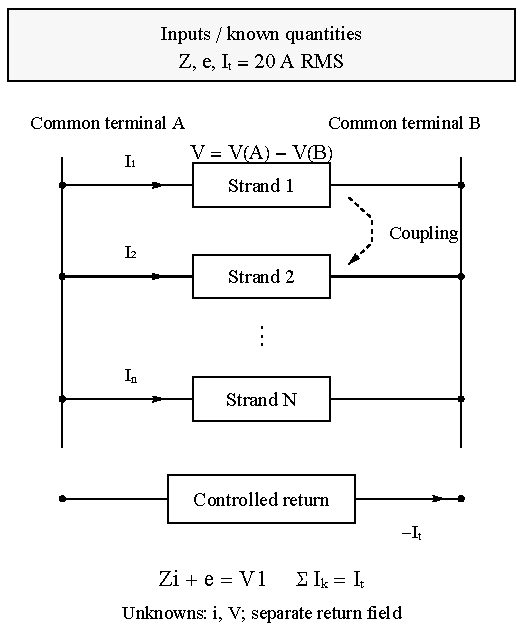
\includegraphics[width=\linewidth,height=.72\textheight,keepaspectratio]{../../assets/en/common_terminal.pdf}
\caption{Multistrand common terminals and return. Strands are insulated along their paths and connected in parallel at both ends; their phasor currents follow from the common voltage and total-current constraints. The coupling matrix Z and excitation term e contain the impedance and field contributions retained by the model. The controlled return carries the opposite total current and has its own terminal field. Known inputs and unknown currents and voltage are identified.}
\label{fig:common_terminal}
\end{figure}

% block-id: 04.figure.coax640_currents
\hypertarget{04.figure.coax640_currents}{}
\begin{figure}[!htbp]
\centering
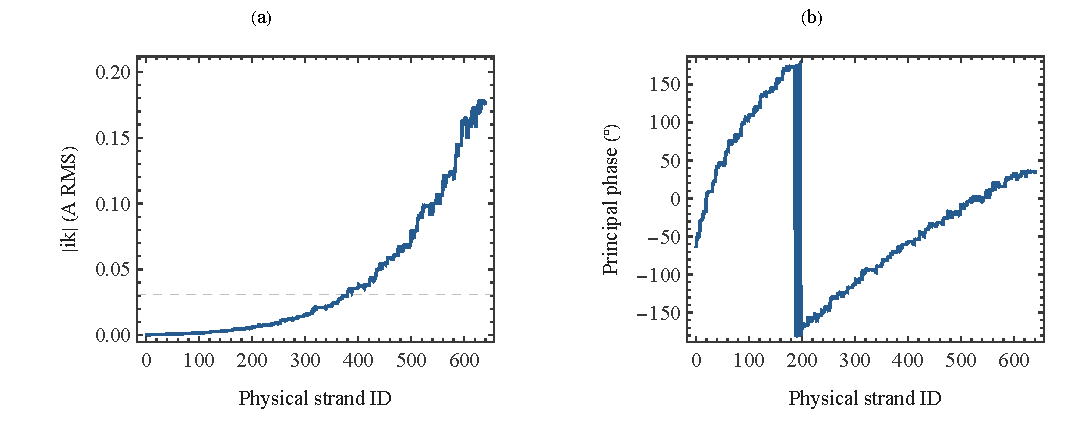
\includegraphics[width=\linewidth,height=.72\textheight,keepaspectratio]{../../assets/en/coax640_currents.pdf}
\caption{640-strand common-terminal complex current sharing. (a) Magnitude; (b) phase, ordered by physical strand identity. A dashed line marks the comparison reference It/N. Magnitude and phase use identical physical strand numbering.}
\label{fig:coax640_currents}
\end{figure}

% block-id: 04.figure.coax640_fields
\hypertarget{04.figure.coax640_fields}{}
\begin{figure}[!htbp]
\centering
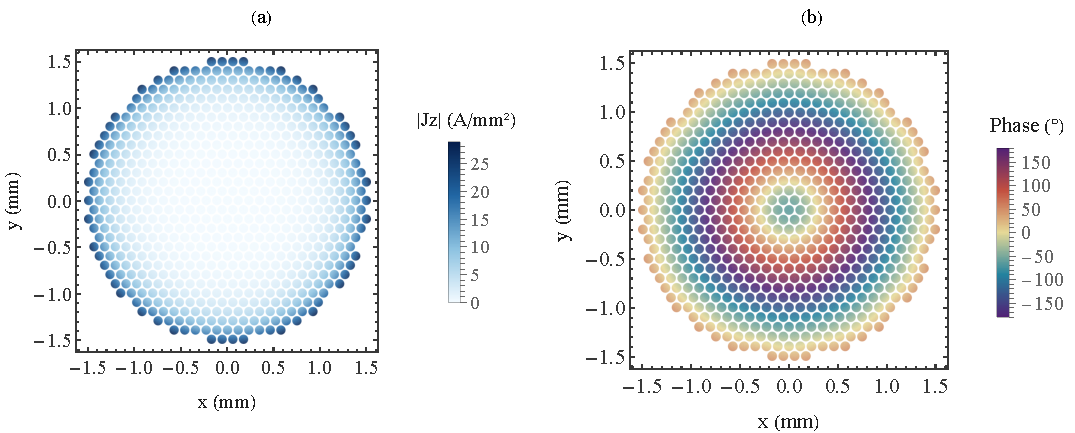
\includegraphics[width=\linewidth,height=.72\textheight,keepaspectratio]{../../assets/en/coax640_fields.pdf}
\caption{640-strand two-dimensional cross-sectional current density. (a) RMS magnitude; (b) phase, with material markers identifying strands. Current is reconstructed as Jz=σ(v−u) from original nodal and terminal fields. Independent power uses linear-triangle mass integration, while visualization samples cell centers.}
\label{fig:coax640_fields}
\end{figure}

% block-id: 04.figure.coax640_mesh
\hypertarget{04.figure.coax640_mesh}{}
\begin{figure}[!htbp]
\centering
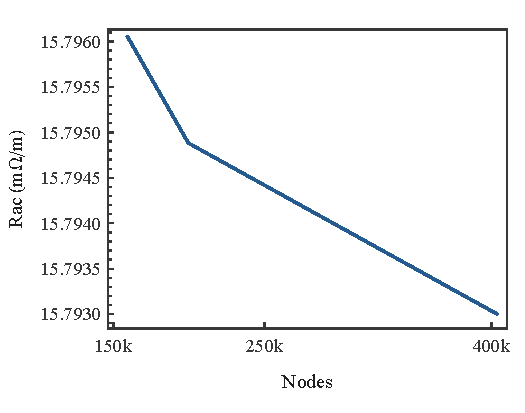
\includegraphics[width=\linewidth,height=.72\textheight,keepaspectratio]{../../assets/en/coax640_mesh.pdf}
\caption{640-strand mesh and boundary sensitivities. Mesh, return, and exterior tests each vary one factor. Variation is normalized from resistance differences between the specified adjacent cases. Mesh, return distance, and exterior size use separate sequences.}
\label{fig:coax640_mesh}
\end{figure}
